\documentclass[12pt]{article}

\usepackage{sbc-template}
\usepackage{graphicx,url}
\usepackage[utf8]{inputenc}
\usepackage[T1]{fontenc}
\usepackage[brazil]{babel}
\usepackage{booktabs}
\usepackage{tabularx}

\sloppy

% Números medidos na versão final. Cada um vem de uma fonte que se repete com um
% comando, anotado ao lado; mudou a medição, muda aqui e só aqui.
\newcommand{\testesContratos}{68}      % pnpm --filter @achei/contratos test
\newcommand{\testesApiUnidade}{90}     % pnpm --filter @achei/api test:unidade
\newcommand{\testesApiIntegracao}{253}  % pnpm --filter @achei/api test:integracao
\newcommand{\testesApp}{237}           % pnpm --filter @achei/mobile test
\newcommand{\testesEdois}{6}         % pnpm e2e (Playwright na versão web)
\newcommand{\testesTotal}{648}
\newcommand{\cargaPnoventaecinco}{26~ms} % docs/qualidade/carga.md
\newcommand{\cargaRequisicoes}{435}
\newcommand{\cargaVintemilPnoventaecinco}{7,7~s}
\newcommand{\cargaVintemilRequisicoes}{10}
\newcommand{\cargaErros}{0\%}
\newcommand{\publicacaoBytes}{902.470~bytes}     % teste RNF2 em packages/contratos

\title{Achei um Bicho: um mural georreferenciado para reencontrar\\ cães e gatos perdidos em Santarém-PA}

\author{Bruna Kellen\inst{1}, Murilo Falcão\inst{1}, Rafael Nobre\inst{1}}

\address{Universidade Federal do Oeste do Pará (UFOPA)\\
  Santarém -- PA -- Brasil
  \email{\{brunakellen1503,falcao.murilo4\}@gmail.com, rafael@rnobre.dev}
}

\begin{document}

\maketitle

\begin{abstract}
  In Santarém, Pará, the news that a dog went missing and the news that a dog
  was found usually circulate on the same day, in different WhatsApp groups,
  and nobody compares them. This paper presents Achei um Bicho, a geolocated
  board of lost and found dogs and cats that compares the declared attributes
  and the distance between cases and explains, in plain words, what matched and
  what did not. Contact between the parties opens only after the case owner
  checks answers to private questions. We describe the requirements, the
  architecture built on free services, the deterministic pairing rules and the
  test-first process, and we report what was measured in the software. A field
  study with local animal protectors is left as future work.
\end{abstract}

\begin{resumo}
  Em Santarém, Pará, a notícia de que um cachorro sumiu e a de que um cachorro
  foi achado costumam circular no mesmo dia, em grupos de WhatsApp diferentes,
  sem que ninguém as compare. Este artigo apresenta o Achei um Bicho, um mural
  georreferenciado de cães e gatos perdidos e encontrados que compara os
  atributos declarados e a distância entre os casos e explica, em palavras, o
  que bateu e o que não bateu. O contato entre as partes só abre depois que
  quem publicou confere as respostas a perguntas que só o tutor sabe responder.
  Descrevemos os requisitos, a arquitetura montada sobre serviços gratuitos, as
  regras determinísticas de pareamento e o processo guiado por testes, e
  relatamos o que foi medido no software. O estudo de campo com protetores
  locais fica como trabalho futuro.
\end{resumo}

\section{Introdução}

Quem perde um cachorro em Santarém publica a foto num grupo de WhatsApp do
bairro. Quem encontra um cachorro na rua publica em outro grupo, às vezes no
mesmo dia. As duas mensagens descem na conversa e somem, e a comparação entre
elas depende de alguém, por acaso, estar nos dois grupos e lembrar das duas
fotos.

A literatura sobre animais perdidos aponta para a vizinhança. Num estudo com
domicílios norte-americanos, a busca pelo bairro e a volta espontânea foram os
caminhos mais comuns de reencontro de cães \cite{weiss2012}. Nos dados do abrigo
público de Dallas, 70\% dos cães devolvidos aos tutores estavam a no máximo uma
milha (1,6~km) de casa, e 42\% a um quarteirão \cite{kremer2021}. Com gatos, 75\%
dos animais achados estavam a menos de 500~m do ponto de fuga \cite{huang2018}.
Um aviso para a cidade inteira, portanto, gasta a atenção de quem mora longe e
pouco ajuda.

O Achei um Bicho parte dessa observação. É um mural de casos de cães e gatos
perdidos e encontrados que abre em volta de quem está olhando, num raio inicial
de 1,6~km. Quando alguém publica um caso, o sistema procura casos do outro lado
(perdido contra encontrado) e mostra cada par com o que bateu e o que não bateu,
sem nota nem porcentagem. A decisão de que é o mesmo animal é sempre de uma
pessoa. O telefone das partes só aparece depois que quem publicou confere as
respostas a três perguntas que só o tutor sabe responder.

Este artigo descreve o sistema e o processo usado para construí-lo na disciplina
de Laboratório de Desenvolvimento de Software da UFOPA. As contribuições são: um
conjunto de regras de pareamento que cabe numa frase cada e pode ser mostrado na
tela; um desenho de privacidade em que o ponto exato e o contato não saem da API
por construção; e o relato de um processo em que diagramas, restrições do banco
e documentação são gerados de uma fonte única, com testes que reprovam quando
ficam para trás.

\section{Trabalhos relacionados}

A identificação permanente é a ferramenta mais estudada para devolver animais. Num
levantamento em 53 abrigos, 74\% dos donos de cães com microchip foram
encontrados, e a principal falha foi o telefone cadastrado errado ou desligado
\cite{lord2009}. Esse resultado sustenta uma escolha deste trabalho: em vez de
depender de cadastro prévio, que envelhece, o sistema trabalha com o caso
publicado no momento da perda ou do achado.

O papel das redes sociais na busca já foi descrito. Perfis dedicados a animais
desaparecidos e furtados usam imagem, relato emocional e compartilhamento em massa
para tornar o animal visível, e o mesmo estudo documenta furto de animais para
cobrar resgate \cite{arathoon2024}. O Achei um Bicho prefere avisar quem mora perto a
espalhar o caso pela cidade, e põe uma verificação antes do contato, pensada
contra o golpe em que alguém diz ter achado o animal para cobrar a devolução.

Programas baseados na comunidade reforçam a escala de bairro. Um programa de um
abrigo nos Estados Unidos devolveu gatos achados a uma distância mediana de
0,27~km de casa \cite{dalrymple2025}. O raio inicial do mural e o limite de
distância das regras de pareamento vêm desses números, com a ressalva de que
ainda precisam ser confirmados em Santarém.

No lado técnico, a consulta por raio sobre um índice espacial é o núcleo do
mural. Avaliações do PostGIS mostram que consultas espaciais sem índice crescem
muito mais com o tamanho da tabela do que as indexadas com R-tree sobre GiST
\cite{nguyen2009}. Para a localização publicada, o trabalho sobre
geo-indistinguibilidade formaliza a proteção do ponto exato pela publicação de
uma área com ruído controlado \cite{andres2013}. O sistema adota uma versão mais
simples e determinística, discutida na Seção~\ref{sec:privacidade}.

\section{O sistema}

\subsection{Requisitos}

O produto tem nove funcionalidades, de F1 a F9. Publicar caso perdido (F1) e
encontrado sem criar conta (F2); ver o mural por proximidade (F3); abrir um caso e
avisar que viu o animal (F4); receber pistas de pareamento (F5); reivindicar o
animal respondendo às perguntas de verificação (F6); liberar o contato só depois
de conferir as respostas (F7); encerrar o caso com o desfecho, com cobrança e
expiração do caso parado (F8); e publicar sem conexão (F9). A
Tabela~\ref{tab:requisitos} resume as regras que mais pesam no desenho.

\begin{table}[ht]
\centering
\caption{Regras de negócio e requisitos não funcionais que orientaram o desenho}
\label{tab:requisitos}
\begin{tabularx}{\textwidth}{lX}
\toprule
RN2 & Publicar caso de animal encontrado não exige conta \\
RN4 & Respostas de verificação são visíveis apenas para o autor do caso \\
RN5 & Dados de contato só aparecem após liberação explícita do autor \\
RN6 & Pareamento compara apenas atributos declarados, sem inferência \\
RN8 & Caso parado é cobrado e, sem resposta, expira \\
RN10 & Localização é sempre publicada como área aproximada \\
RNF2 & Publicar um caso consome menos de 1~MB de dados \\
RNF4 & Nenhum dado pessoal aparece antes da liberação \\
RNF5 & Contraste mínimo AA, para uso na rua sob sol \\
\bottomrule
\end{tabularx}
\end{table}

\subsection{Arquitetura}

A Figura~\ref{fig:arquitetura} mostra as três peças. O aplicativo é escrito em
React Native com Expo e roda como APK no Android e como versão web, que atende o
iPhone sem passar pela loja. A API é escrita em NestJS, com Prisma, e roda num
contêiner no Render. O banco é PostgreSQL com a extensão PostGIS, hospedado no
Neon. Os três serviços têm plano gratuito sem cartão de crédito, uma restrição do
projeto. A integração contínua roda os tipos e todos os testes a cada envio ao
repositório e dispara, uma vez por dia, a tarefa de cobrança e expiração.

\begin{figure}[ht]
\centering
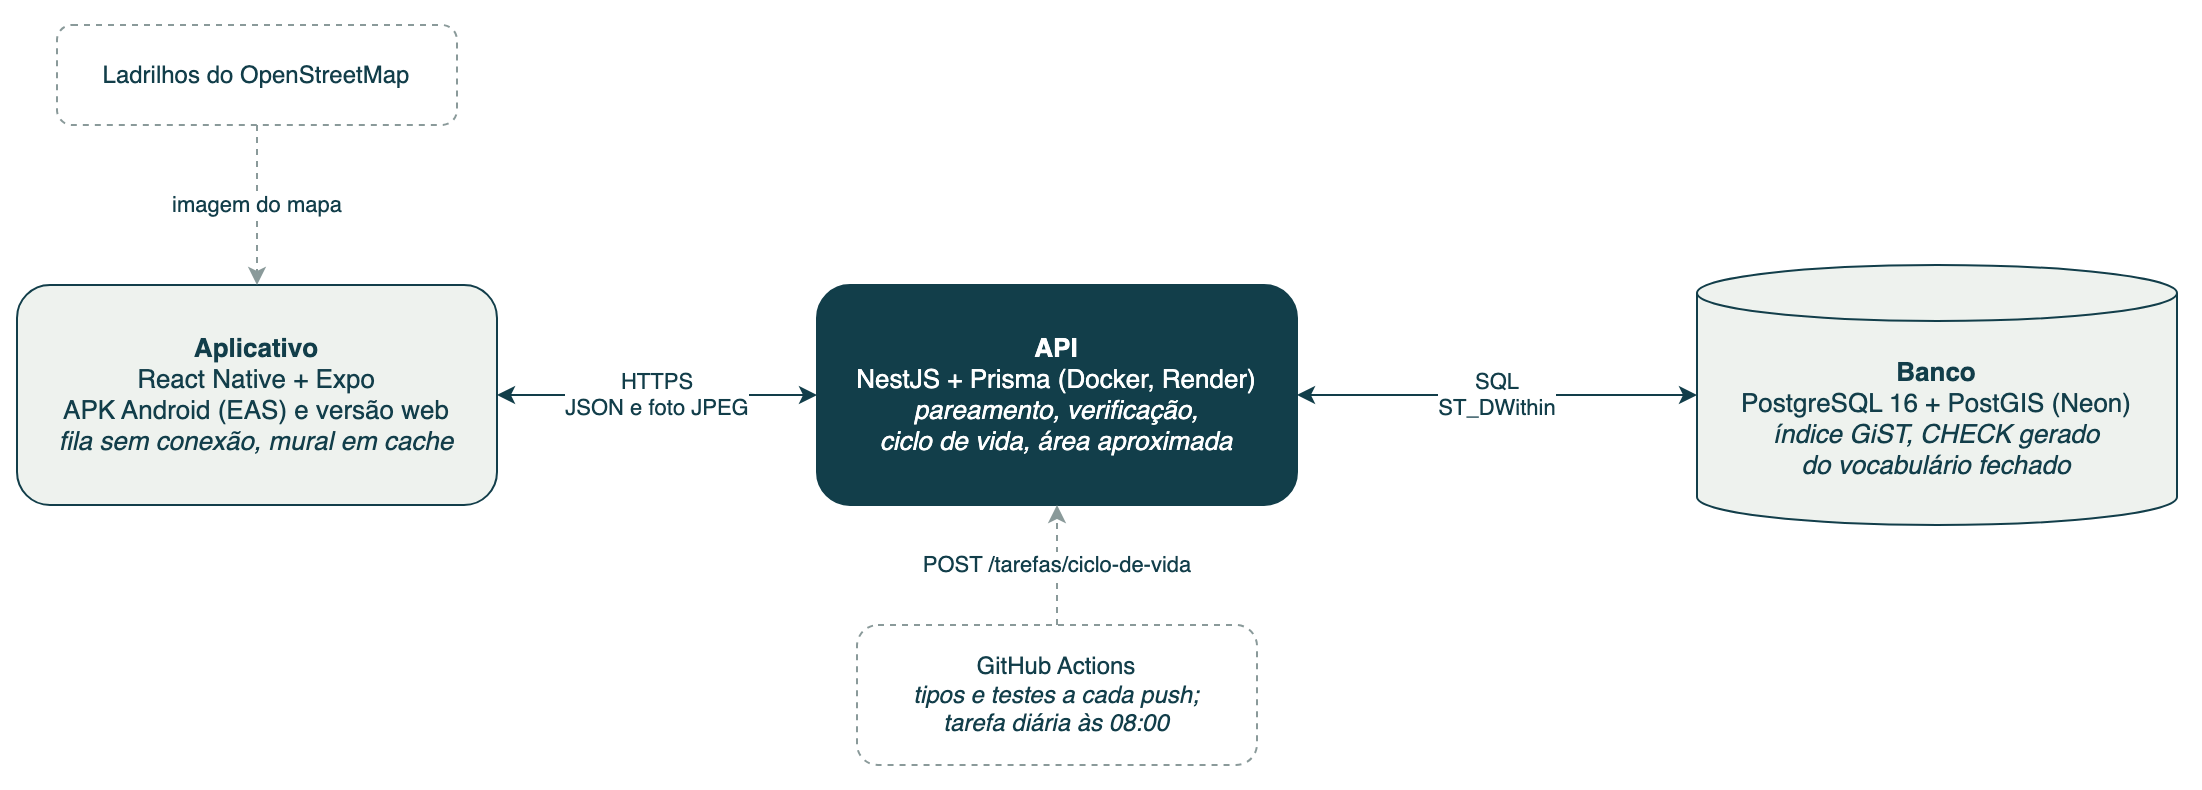
\includegraphics[width=.95\textwidth]{figuras/arquitetura.png}
\caption{Arquitetura do Achei um Bicho}
\label{fig:arquitetura}
\end{figure}

O mapa não usa biblioteca nativa. O aplicativo monta a imagem com ladrilhos do
OpenStreetMap e desenha o círculo da área por cima, o que funciona igual no
aparelho, na web e no Expo Go. O preço é não ter arrastar nem zoom, aceitável
para uma tela que só precisa mostrar a região. Tocar no mapa abre o Google Maps
centrado na região, sem marcação, pelo mesmo motivo de privacidade da
Seção~\ref{sec:privacidade}.

\subsection{Mural por proximidade}

O mural é uma consulta por raio no banco. A condição usa \texttt{ST\_DWithin},
que aproveita o índice GiST sobre a coluna geográfica; a distância exibida usa
\texttt{ST\_Distance}, que fica só na lista de colunas. Trocar as duas de lugar
faz o banco percorrer a tabela inteira, e é por isso que o modelo de dados
declara o índice como obrigatório. O raio começa em 1,6~km e cresce, por um
botão, em degraus até 5~km.

\subsection{Pareamento explicado}
\label{sec:pareamento}

Ao publicar, o sistema procura candidatos do lado oposto, da mesma espécie, ainda
abertos e a até 5~km. Para cada par, compara cinco itens e guarda separadamente o
que bateu e o que não bateu (Tabela~\ref{tab:pareamento}). As pistas aparecem
ordenadas pelo número de coincidências e, no empate, pela distância. Nenhum
número sai daí para a tela. A tela mostra cada item com uma frase, por exemplo
``Os dois com coleira'' ou ``Achado 5 dias antes do sumiço informado''.

\begin{table}[ht]
\centering
\caption{Regras de pareamento; cada uma aparece na tela como uma frase}
\label{tab:pareamento}
\begin{tabularx}{\textwidth}{lX}
\toprule
Porte & Bate quando os dois declaram o mesmo porte \\
Cor & Bate quando a cor dominante é a mesma \\
Coleira & Bate quando os dois dizem o mesmo; ``não deu para ver'' não conta \\
Distância & Bate até 1,6~km entre os pontos \\
Tempo & Bate se o achado foi de um dia antes a 30 dias depois do sumiço \\
\bottomrule
\end{tabularx}
\end{table}

A escolha por regras explicáveis em vez de um modelo de pontuação foi deliberada.
Uma porcentagem não diz ao tutor o que conferir; ``a cor bateu, a coleira não''
diz. A regra também é defensável diante de quem pergunta por que dois casos foram
aproximados, e cabe no prazo de uma disciplina.

\subsection{Verificação e contato mediado}

Quem publica cadastra três perguntas com as respostas, por exemplo ``Que sinal
ele tem que não aparece na foto?''. Quem acha que o animal é seu responde às três
no aplicativo; no caso de um animal perdido, é quem diz ter achado que responde. O
autor do caso vê as respostas ao lado das que cadastrou e decide. O aplicativo
diz em texto que não decide de quem é o animal.

Só depois do aceite os dois lados recebem nome e telefone, e quem está com o
animal informa onde ele está. A tela do contato traz um aviso fixo: não pague para
receber o animal e combine o encontro num lugar público. Quem reivindica não
precisa de conta: recebe um código de acompanhamento, guardado no aparelho, para
voltar e ver a decisão. Há um teto de reivindicações pendentes por caso, o mesmo
telefone não reivindica de novo um caso que já o recusou, e o autor vê quantas
denúncias o telefone já recebeu antes de aceitar.

\subsection{Privacidade por construção}
\label{sec:privacidade}

O ponto exato do caso nunca sai da API. O que se publica é uma área: um círculo
de 300~m cujo centro é deslocado do ponto real por uma distância entre 25\% e 75\%
do raio. O deslocamento é sempre o mesmo para o mesmo caso: se fosse sorteado a
cada leitura, bastaria consultar o caso várias vezes e tirar a média para achar o
ponto. Ele vem de um HMAC do identificador do caso com um segredo do servidor. É uma
proteção mais fraca que a geo-indistinguibilidade \cite{andres2013}, mas suficiente
para o objetivo de não expor a casa de quem acolheu o animal, e não exige parâmetro
de privacidade que o usuário precise entender.

As duas falhas desse desenho apareceram na revisão independente. Na primeira versão
o deslocamento vinha só do identificador, que é público; com o código aberto,
qualquer pessoa podia refazer a conta e subtrair o deslocamento do centro publicado.
O segredo fechou essa porta. A segunda era mais simples. O mural informava a distância
de cada caso até o ponto real, e quem consulta escolhe o centro da busca: três
consultas de lugares diferentes davam o ponto por trilateração. Hoje a distância, a
ordem e a contagem do mural, e a distância entre casos nas pistas, saem do centro
publicado.

O mesmo cuidado vale para os demais dados. O código de edição e o de
acompanhamento são guardados só como HMAC com segredo do servidor. Quem avisa que
viu o animal não tem o ponto revelado: o autor vê a distância e o bairro. A foto é
regravada no aparelho sem os metadados da câmera, que guardam a coordenada, e a API
descarta de novo esses segmentos do JPEG. Texto livre público que traz telefone ou
link é recusado, para não furar o contato mediado. Trinta dias depois de encerrado,
o caso sai do ar e perde nome e telefone das partes, as respostas de verificação, os
avisos de quem viu o animal e o ponto exato, trocado pelo centro da área que já
estava publicada. Sair do ar faz parte da proteção: servir de novo a área de um caso
anonimizado aplicaria um segundo deslocamento sobre o primeiro, e quem tivesse lido as
duas versões chegaria ao ponto real por diferença.

\subsection{Ciclo de vida}

O caso perdido nasce ``procurando'' e o encontrado, ``abrigado por alguém''. A
Figura~\ref{fig:estados} mostra as transições, declaradas uma única vez no código e
lidas tanto pela API quanto pelo gerador do diagrama. Um caso sem ação do autor
por nove dias recebe um pedido de confirmação; sem resposta até o 15º dia, expira e
sai do mural. Encerrar exige informar o desfecho (voltou para casa, foi adotado ou
não foi encontrado), que é o dado necessário para medir, no futuro, quantos
reencontros o sistema ajudou a produzir.

\begin{figure}[ht]
\centering
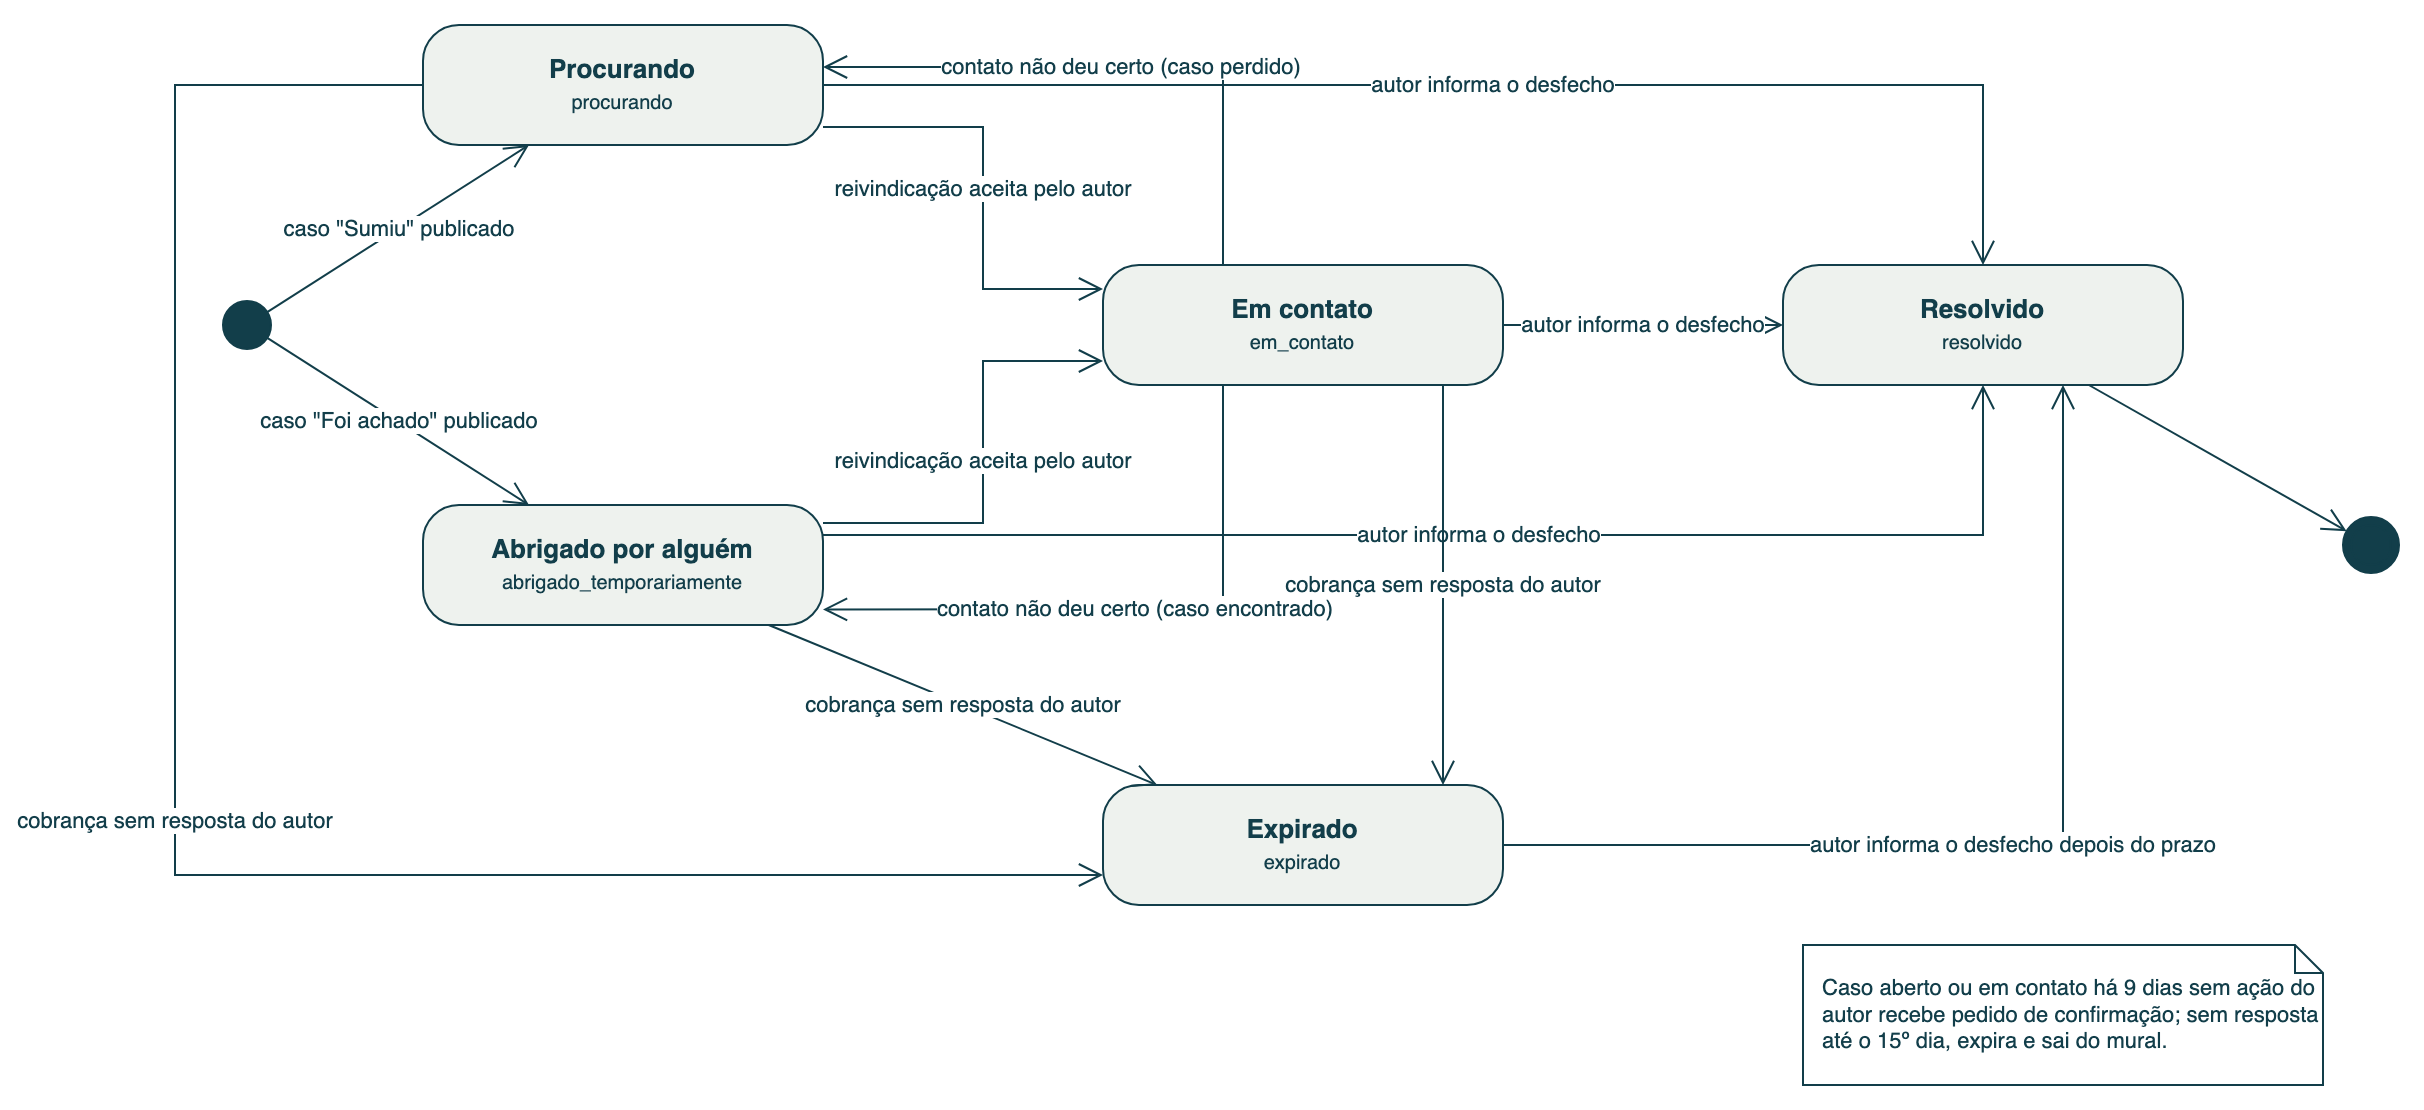
\includegraphics[width=\textwidth]{../uml/estados.png}
\caption{Estados do caso, gerados das transições declaradas no código}
\label{fig:estados}
\end{figure}

\subsection{Publicar sem conexão}

Fora do centro de Santarém a conexão móvel cai com frequência. A publicação passa
sempre por uma fila guardada no aparelho: a foto já reduzida, os dados e um
identificador gerado no próprio celular. Sem conexão, a tela diz que o caso está
guardado e sobe sozinho quando a internet voltar, e nunca diz ``publicado'' antes
da confirmação do servidor. Se a confirmação se perder e a fila reenviar, a API
reconhece o identificador e devolve o mesmo caso, sem criar outro. O mural e os
casos já abertos ficam guardados e continuam legíveis sem conexão.

\section{Processo de desenvolvimento}

O trabalho seguiu práticas da Programação Extrema \cite{beck2004}, com uma regra
central: nenhuma linha de código de produção antes do teste que ela faz passar, e
o teste precisa ser visto falhando antes. Cada comportamento entrou no histórico
em dois registros, o do teste e o da implementação.

Uma segunda regra organizou a documentação. Alguns fatos precisam concordar em
vários lugares: os valores de porte, cor e coleira aparecem no tipo TypeScript, na
restrição CHECK do banco, nos botões das telas, na documentação e neste artigo, e
o compilador só alcança o primeiro. Esses valores foram declarados uma vez, num
manifesto. A migração do banco, os rótulos das telas, a tabela da documentação e
os diagramas de classes e de estados são gerados a partir dele, e testes comparam
o que está em disco com o que o código geraria. Quando alguém acrescenta um valor
e esquece de gerar, o teste reprova.

A Tabela~\ref{tab:testes} mostra os testes automatizados da versão final. Os de
integração rodam contra PostgreSQL com PostGIS de verdade, num contêiner, e não
contra imitação do banco. A integração contínua reprova o envio se qualquer um
falhar.

\begin{table}[ht]
\centering
\caption{Testes automatizados na versão final}
\label{tab:testes}
\begin{tabular}{lr}
\toprule
Contratos e vocabulário & \testesContratos \\
API, unidade & \testesApiUnidade \\
API, integração com PostgreSQL e PostGIS & \testesApiIntegracao \\
Aplicativo, regras de tela & \testesApp \\
\midrule
Subtotal da suíte & \testesTotal \\
Ponta a ponta na versão web & \testesEdois \\
\midrule
\bottomrule
\end{tabular}
\end{table}

Os testes não bastaram. Três defeitos só apareceram quando o aplicativo foi
instalado num celular de verdade, e nenhum deles aparecia na versão web. O
servidor de mapas bloqueava os ladrilhos pedidos sem identificação do aplicativo.
O componente de imagem do Android descartava os cabeçalhos da requisição quando a
fonte não vinha numa lista. E a biblioteca de rede da versão do Expo usada
recusava o formato antigo de envio de arquivo, de modo que a foto nunca chegava ao
servidor. Cada defeito ganhou um teste de regressão antes do conserto, e a lição
virou regra do projeto: antes de apresentar, todos os fluxos passam pelo APK
instalado. A passada final achou mais um. Com a fila aberta, o caso subia assim
que a rede voltava, mas a tela continuava dizendo que esperava conexão. Esse se
reproduziu no navegador e ganhou um teste de ponta a ponta.

As funcionalidades da segunda metade (verificação, contato, ciclo de vida e
publicação sem conexão) foram feitas em frentes paralelas, e cada uma passou por uma
revisão independente antes de entrar na versão final. A revisão devolveu as quatro
na primeira rodada. Entre o que ela achou estão dois aceites simultâneos que
liberariam o telefone do autor a duas pessoas, uma fila que apagava em silêncio um
caso publicado sem sinal quando o servidor o recusava e o deslocamento da área
aproximada descrito na Seção~\ref{sec:privacidade}. Cada achado voltou com um teste
que reprova o defeito.

\section{Avaliação}

Esta seção relata o que foi medido no software. Ela não mede o efeito do sistema
sobre reencontros, que depende de uso real e é discutido na
Seção~\ref{sec:limitacoes}.

\textbf{Carga do mural.} Com 200 casos em volta de um ponto, 26 deles dentro do raio
de 1,6~km, a consulta do mural atendeu \cargaRequisicoes{} requisições por segundo
com p95 de \cargaPnoventaecinco{} e taxa de erro de \cargaErros{}, medidos com k6
durante 30~segundos com até 50 usuários virtuais, contra a API compilada. Com
20.000 casos, densidade que Santarém não deve ter, o p95 subiu para
\cargaVintemilPnoventaecinco{}, muito acima da meta de 300~ms. O custo vem de uma escolha
de privacidade: como o mural decide tudo pelo centro publicado, e esse centro sai de um
HMAC com o segredo do servidor, a API traz do banco todos os casos abertos até 5~km e
calcula a área de cada um antes de filtrar, ordenar e contar. Na densidade de Santarém
isso não aparece; se aparecer, o caminho é calcular o deslocamento no próprio banco.
Antes, a medição com 20.000 casos já tinha revelado um plano de consulta ruim: o banco
estimava poucas linhas para o filtro de distância e comparava cada local com cada caso,
8,8~s por consulta, que caíram para 0,5~s com a busca do caso de cada local pelo índice.
A medição foi feita num notebook, com banco e gerador de carga na mesma máquina; ela
mede a consulta, não o serviço gratuito onde a API está hospedada.

\textbf{Consumo de dados (RNF2).} A maior publicação aceita pela API, somada a uma
foto no limite de tamanho, ocupa \publicacaoBytes{}, abaixo de 1~MB. O aplicativo
reduz a foto para 1080 pixels no lado maior antes do envio.

\textbf{Contraste (RNF5).} Todos os pares de cor de texto e fundo do tema passam
pelo critério AA da WCAG, conferido por teste automatizado.

\textbf{Vazamento de dados (RNF4).} Testes de integração percorrem as rotas
públicas e verificam que nenhum corpo de resposta contém telefone, resposta de
verificação, código ou ponto exato antes da liberação.

\textbf{Pareamento.} Um cenário de demonstração, também coberto por teste,
publica a partir do campus um cachorro caramelo de porte médio, com coleira, que
sumiu na véspera. O sistema devolve três pistas: o caso achado a 1,2~km, com
coleira, bate em todos os itens e aparece primeiro; o achado a 670~m, sem coleira,
aparece em segundo apesar de mais perto; e um malhado a 3,4~km aparece por último,
com a cor e a distância contra.

\section{Limitações}
\label{sec:limitacoes}

A principal limitação é a ausência de avaliação com usuários. O cronograma previa
uma rodada com protetores de animais de Santarém, que não aconteceu até a entrega
deste artigo. Por isso não há números sobre reencontros, tempo até o reencontro ou
adesão, e as distâncias usadas no pareamento vêm de estudos norte-americanos
\cite{kremer2021,huang2018} que ainda precisam ser confirmados na cidade. Os casos
usados na demonstração são fictícios, com fotos de domínio público.

Há também limites de infraestrutura. A API gratuita dorme depois de 15 minutos sem
uso e leva perto de um minuto para acordar. O código de edição não tem
recuperação: quem o perde e troca de celular perde o controle do caso, porque
recuperar sem conta abriria o caso para qualquer um. E o aplicativo instalável só
existe para Android; no iPhone, o caminho é a versão web.

\section{Conclusão}

O sistema está no ar: a versão web, o APK para Android e a API rodam em serviços
gratuitos, e a cada envio ao repositório os \testesTotal{} testes automatizados
são executados. A aposta do produto é que um mural de bairro, que explica cada par e
exige verificação antes do contato, faça o que o grupo de WhatsApp não faz:
cruzar o caso de quem perdeu com o de quem achou. Se faz, ainda não sabemos.

Os próximos passos são a rodada com protetores locais, para alimentar o mural com
casos reais e calibrar os limites de distância e de tempo; uma conta opcional,
oferecida depois da publicação, para recuperar casos em outro aparelho; e a
medição dos desfechos registrados, que vai dizer quantos reencontros passaram
pelo mural.

\bibliographystyle{sbc}
\bibliography{referencias}

\end{document}
